\section{E/B Power Spectra Ratios}

In this section we examine the ratio of power in the scalar EE spectra to the
tensor BB spectra across the inertial multipole range in our simulations.
We compare to the observed E/B ratio reported by \citep{Planck18XI} of
$r \approx 2$ and discuss the effects of various parameters on the value measured. 

\begin{figure}[h]
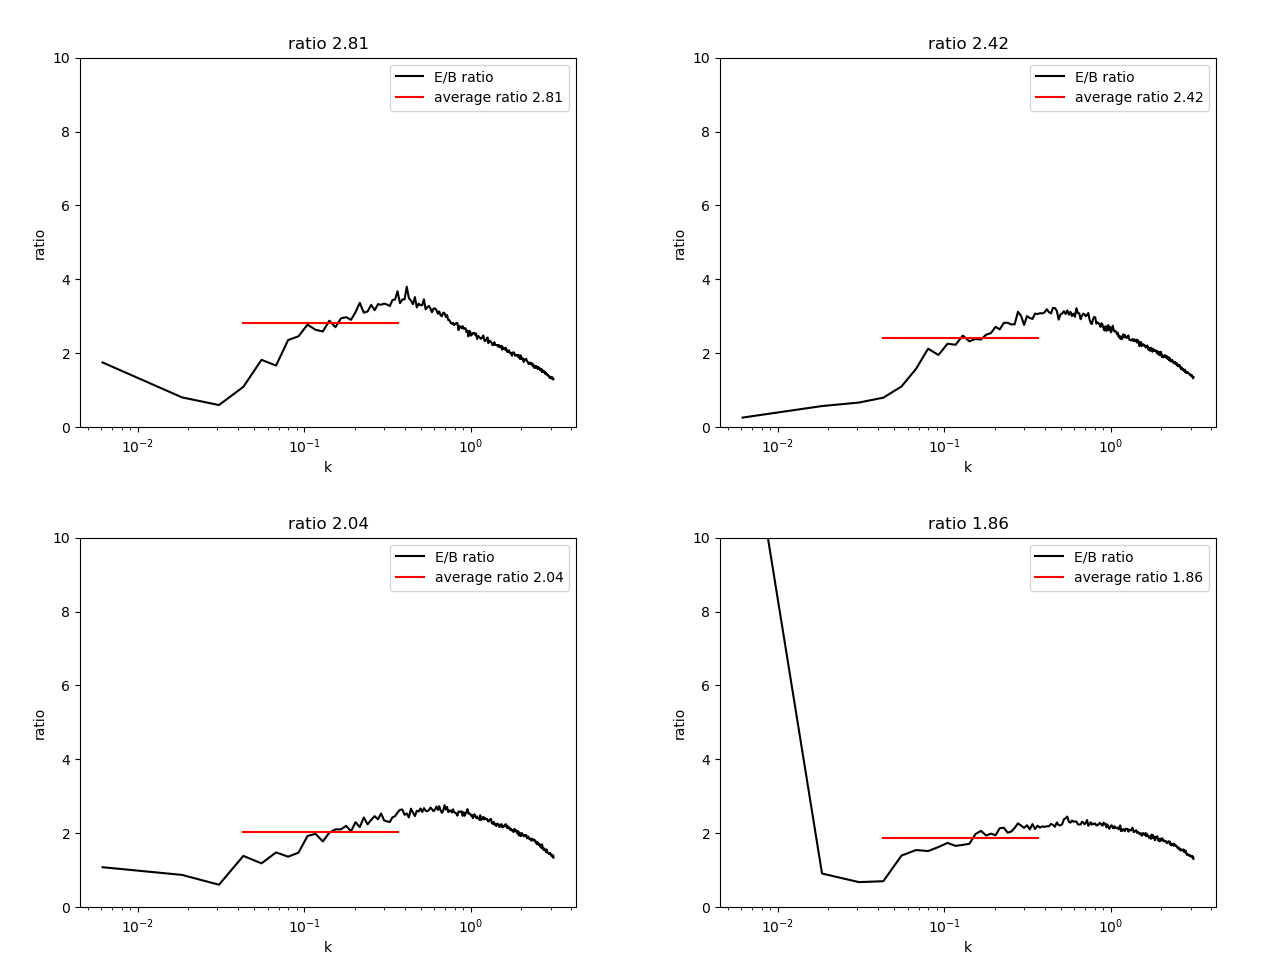
\includegraphics[width=\linewidth]{diff_ratios_x.png}
\caption{Average ratio of EE power to BB power EE/BB across the entire multipole
spectrum for four different simulations in our suite with varying $M_s$ and
$M_a$ parameters. Top Left: $M_s=0.5$ $M_a=2$. Top Right: $M_s=1$ $M_a=2$.
Bottom Left: $M_s=2$ $M_a=2$. Bottom Right: $M_s=3$ $M_a=2$. Each image is taken
with line of sight along the magnetic field and with a red horizontal line
depicting the average power ratio across the fitted inertial multipole range.}
\label{fig:ratio_ms}
\end{figure}

In figure ~\ref{fig:ratio_ms} we can explicitly see the effects of varying the
sonic Mach number $M_s$ on the observed E/B power ratio for a fixed, weak
background magnetic field. In these images we can see two features. The first is
that the ratio of E/B power \emph{decreases} as the ratio $M_{s} / M_{a}$
\emph{increases}. In other words as the sonic pressure increasingly dominates
the magnetic pressure, the ratio of power in EE to BB on average decreases. The
second feature, which is even more apparent in figure ~\ref{fig:ratio_ma} where
the gas pressure is held at a subsonic $M_s = 0.5$, is that the
power ratio as a function of multipole (size scale) becomes much more constant
(flat)  as the Alfven Mach number gets larger, that is to say as the magnetic field
pressure becomes less significant.

\begin{figure}[h]
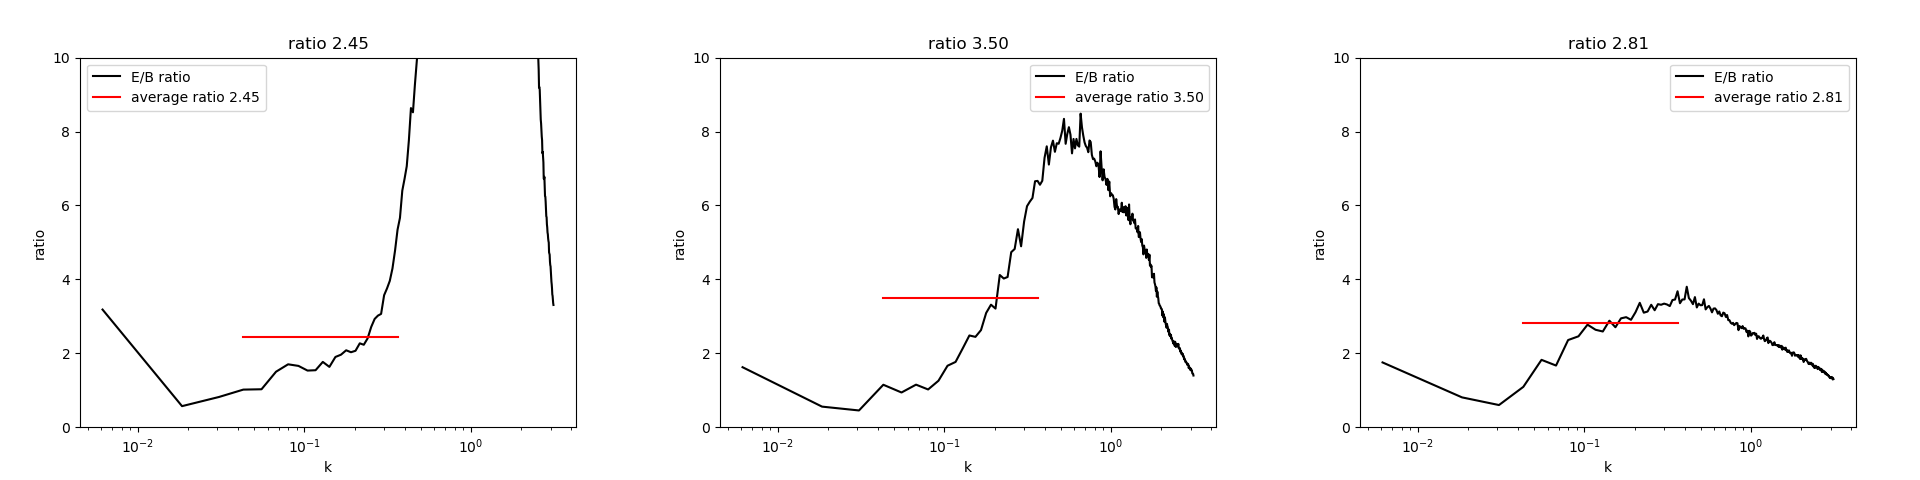
\includegraphics[width=\linewidth]{diff_ratios_x_Ma.png}
\caption{Average ratio of EE power to BB power EE/BB across the entire multipole
spectrum for three different simulations in our suite with varying $M_s$ and
$M_a$ parameters. Left: $M_s=half$ $M_a=half$.
Middle: $M_s=half$ $M_a=1$. Right: $M_s=half$ $M_a=2$. Each image is taken
with line of sight along the magnetic field and with a red horizontal line 
depicting the average power ratio across the fitted inertial multipole range.}
\label{fig:ratio_ma}
\end{figure}

Again the detailed results of our simulation suite including those discussed
above are most easily seen in figure ~\ref{fig:slopes_ratios_param}. Similarly
to the EE and BB slopes, we see that line of sight effects with respect to the
magnetic field orientation range from minimal, when the Alfven Mach number is
high (magnetic field is weak) to significant, when the Alfven Mach number is low
(strong magnetic field). Our results suggest that a super-sonic, super-Alfvenic
flow is the most likely candidate to explain the observed E/B ratios.
